\documentclass[a4paper,12pt]{report}            % [forma A4, taille police] {Type}
    \usepackage[utf8]{inputenc}                
    \usepackage[T1]{fontenc}                        % Codage des fontes TeX
    \usepackage[francais]{babel}
    \usepackage{graphicx}
    \usepackage{wrapfig}
    \usepackage{fancyhdr}
    \usepackage{xcolor}
    \usepackage{hyperref}
    \usepackage{listings}
    \usepackage{fullpage}
    \usepackage{eso-pic}
    \usepackage{titlesec}
    \titleformat{\chapter}[hang]{\bf\huge}{\thechapter}{2pc}{}
    \lstset {numbers=left ,stepnumber=1,firstnumber=0,numberfirstline=true}
    \hypersetup{
        bookmarks=true,         % show bookmarks bar?
        unicode=false,          % non-Latin characters in Acrobat’s bookmarks
        pdftoolbar=true,        % show Acrobat’s toolbar?
        pdfmenubar=true,        % show Acrobat’s menu?
        pdffitwindow=false,     % window fit to page when opened
        pdfstartview={FitH},    % fits the width of the page to the window
        pdftitle={My title},    % title
        pdfauthor={Author},     % author
        pdfsubject={Subject},   % subject of the document
        pdfcreator={Creator},   % creator of the document
        pdfproducer={Producer}, % producer of the document
        pdfkeywords={keyword1, key2, key3}, % list of keywords
        pdfnewwindow=true,      % links in new PDF window
        colorlinks=true,       % false: boxed links; true: colored links
        linkcolor=black,          % color of internal links (change box color with linkbordercolor)
        citecolor=green,        % color of links to bibliography
        filecolor=magenta,      % color of file links
        urlcolor=blue           % color of external links
    }
    
    \author{Samuel HUET \& Thomas COUTANT}
    \title{\huge{Analyseur de Réseaux}}
    
    \begin{document}
\maketitle
\renewcommand{\contentsname}{SOMMAIRE} % Dans le corps du document,avant la commande \tableofcontents.
\tableofcontents

\chapter{Calibrations}
\addcontentsline{toc}{chapter}{Calibrations}

    Afin de mesurer avec précision les paramètres S de notre système, il est nécéssaire de
calibrer l'appareil afin de minimiser au possible les erreurs internes. Mais avant l'étape
de la calibration, nous pouvons déjà brancher le système et regarder sur quelle gamme de
fréquence et sur quelle puissance faut il calibrer. une fois cela fait, nous pouvont aller
dans le menu de calibration en appuyant sur \textbf{CAL}, et voici ce que l'on y trouve :

\begin{center}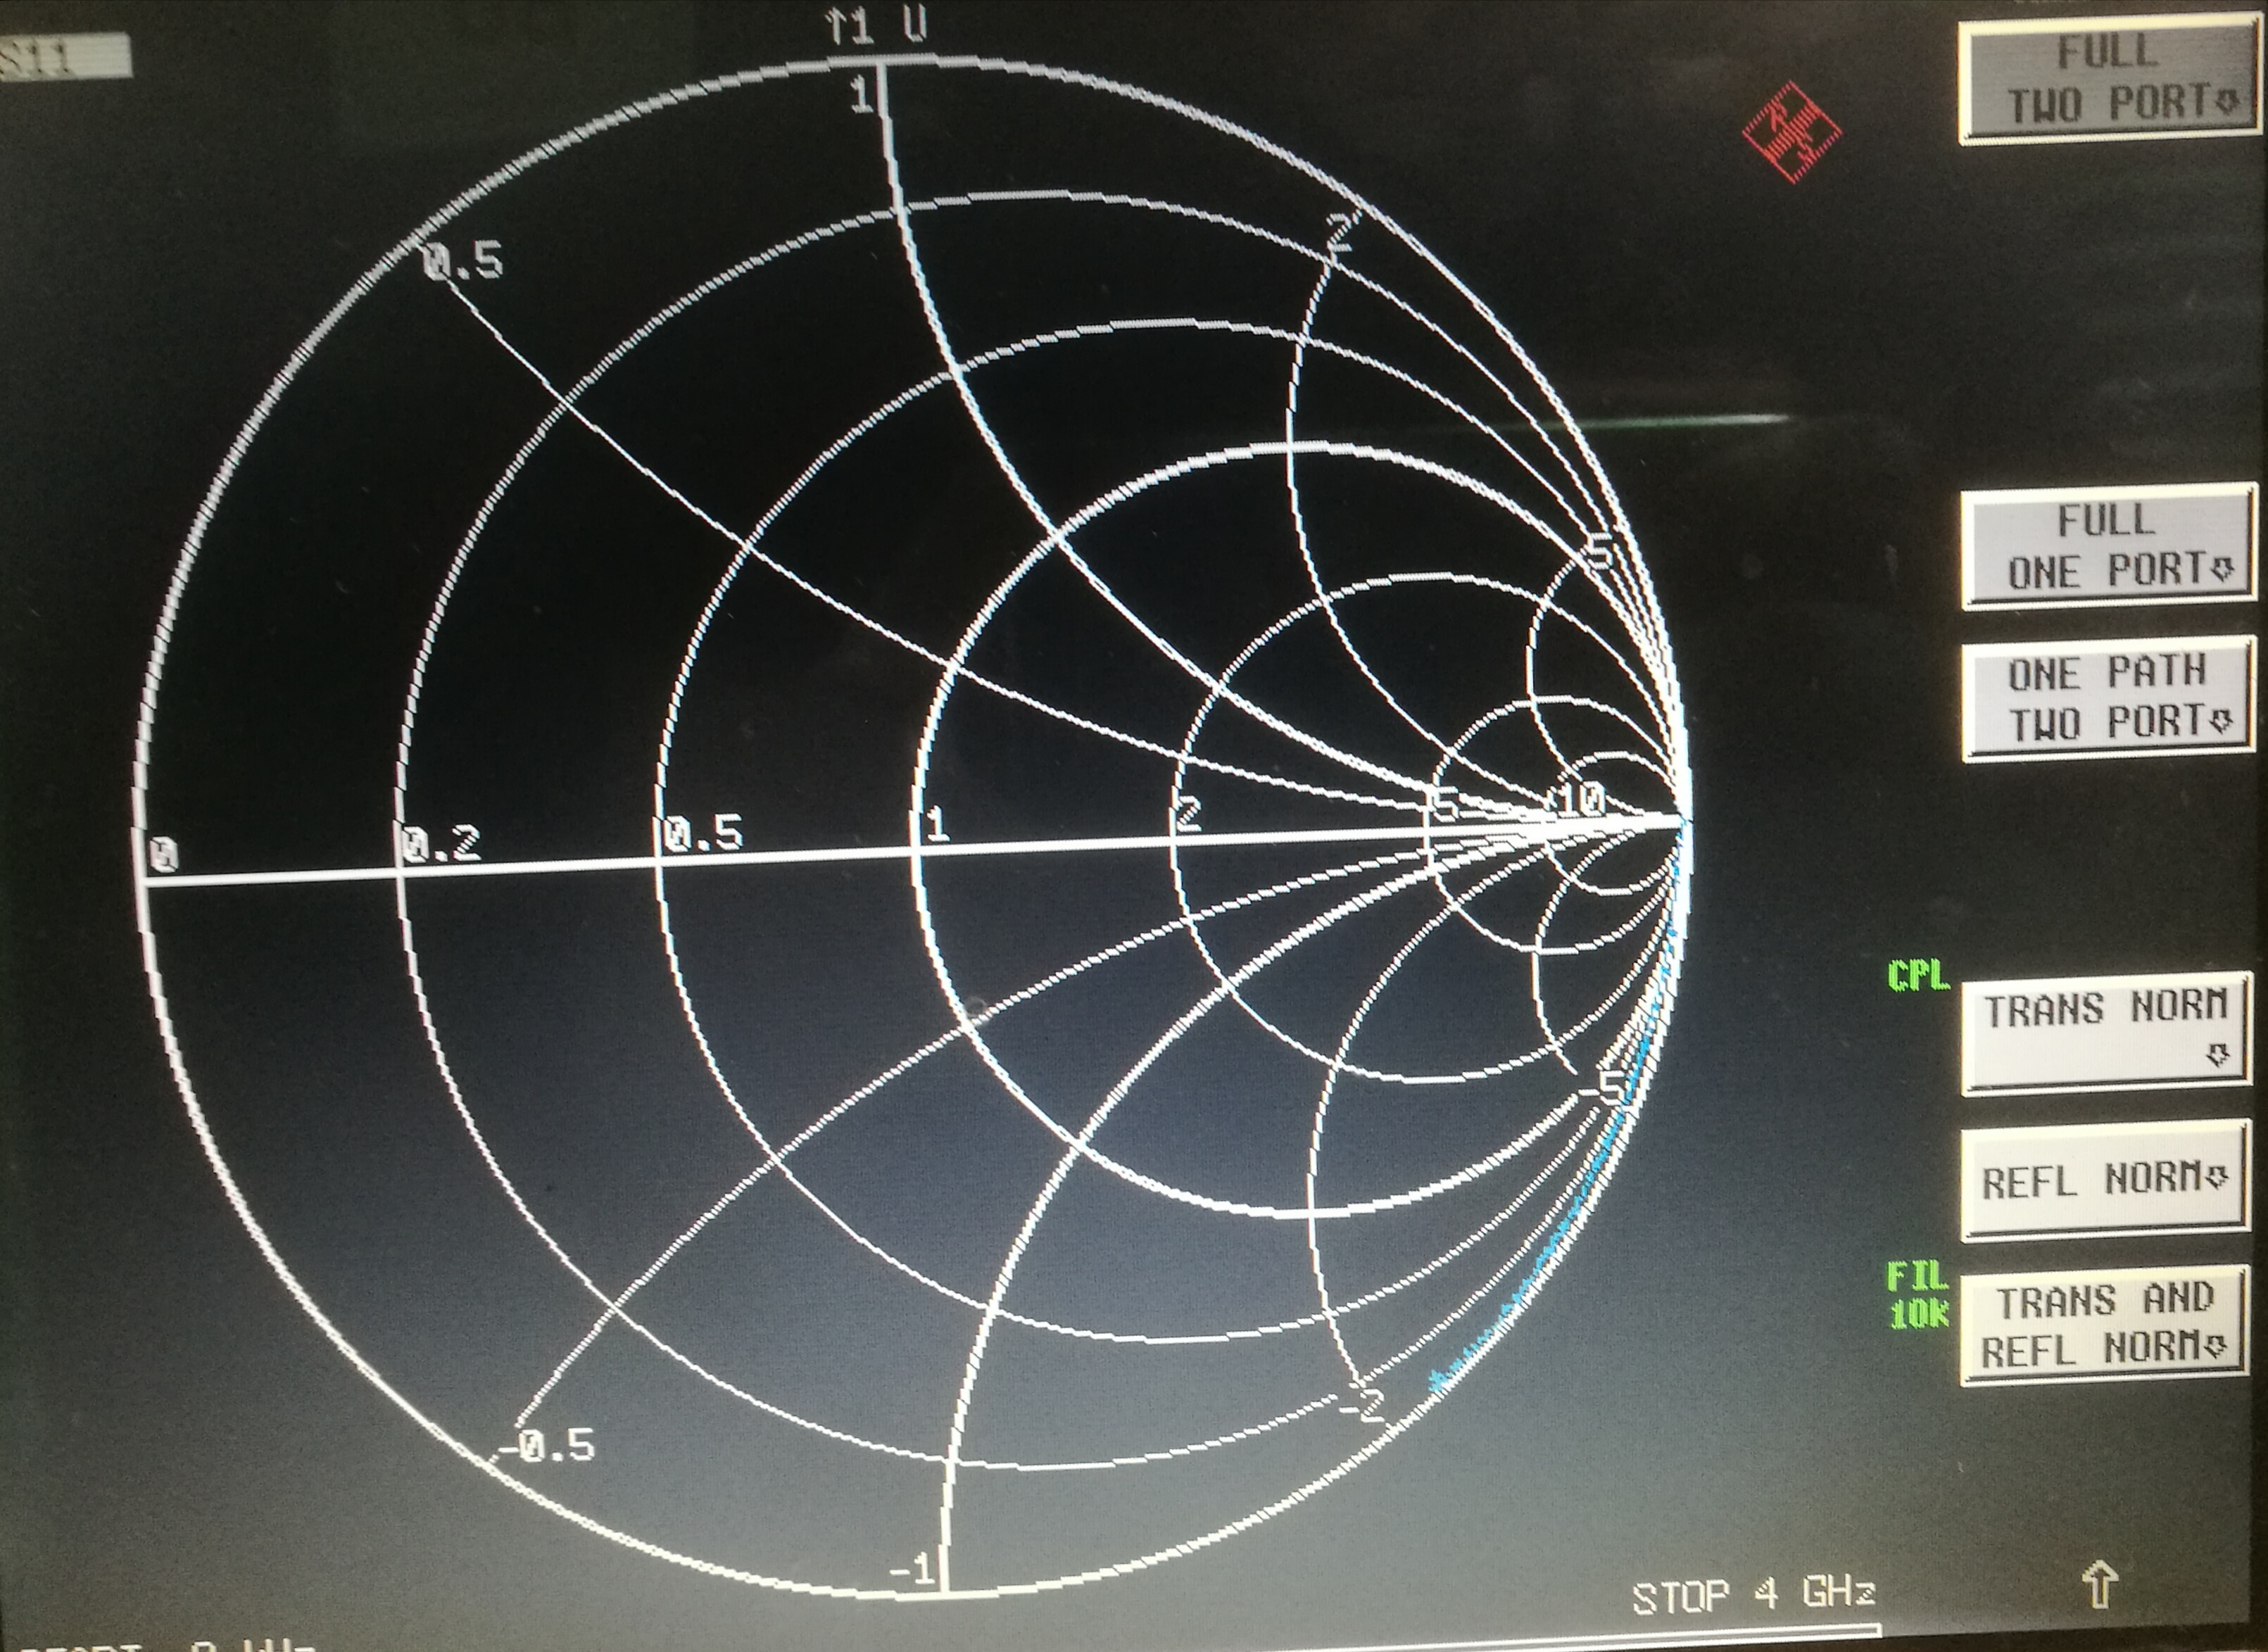
\includegraphics[scale = 0.12]{pic/Calib.jpg}\\ \end{center}

\section{Calibrations possibles}
    Nous pouvons voir 6 boutons qui correspondent en réalité à 6 types de calibration
différentes :
\begin{itemize}
    \item \textbf{FULL TWO PORT} représente une calibration sur les deux ports, donc des 4 paramètres.
        C'est la calibration la plus longue car elle nécéssite de brancher et débrancher sur les deux ports.
    \item \textbf{FULL ONE PORT} ne va calibrer uniquement qu'un seul port, afin de calculer les paramètres
        S11 et S21 (ou S22 et S12)
    \item \textbf{ONE PATH TWO PORT} Ne calibrera que dans le but de mesurer les paramètres S21 et S12.
    \item \textbf{TRANS NORM}
    \item \textbf{REFL NORM}
    \item \textbf{TRANS AND FEFL NORM}
\end{itemize}

    Pour nos mesures, nous avons utilisé la calibration \textbf{FULL TWO PORT} afin
d'analyser le plus de paramètres possible.  

\chapter{Mesures des filtres}
\addcontentsline{toc}{chapter}{Mesures des filtres}

\chapter{Association des filtres}
\addcontentsline{toc}{chapter}{Association des filtres}

\chapter{Diviseur de puissance}
\addcontentsline{toc}{chapter}{Diviseur de puissance}

\chapter{Coupleur}
\addcontentsline{toc}{chapter}{Coupleur}

\end{document}